ABSTRACT

%****************************************
% SAMPLE ABSTRACTS

% Bu çalışmada, ne kadar itici bir kavram olsa da, çöplük olgusunun çirkinlikten güzelliğe ulaşarak estetik bir haz uyandırması amaç edinilmiştir. Iticici gözüken bir konunun resim diliyle anlatımı ile tersine çekici ilginç bir sanat konusu olabileceğinin somutlaştırılması amaçlanmıştır. Sanatçı bir anlamda doğada yaşamda bulunan küçük ayrıntıları, sanatsal bir gözle yaklaşarak gösterebilendir. Resim için konu denince hep bildik tanıdık nesneler, belli bir düzenleme anlayışı (Natürmort) ya da idealize edilmiş konular, temalar akla gelir. Oysa önemsiz gibi gözüken itici karmaşık konular bile sanatsal kaygılarla ele ahnabilmelidir. Önemli olan, bu konalara estetik yaklaşım ve izlenen anlatım yol ve teknikleridir. Özgün baskı dallarından kazı resim (gravür) tekniğinin ele alınan konunun görselleştirilmesinde, anlatımında en uygun teknik olmasıdır. Çünkü her sanatçı kendi doğasına en uygun olan teknik ve malzemelerin olanaklarıyla kendini en rahat biçimde ifade etme olanağı bulur. Kendine özgü bir biçim ve anlatım diliyle dile getirmek gerçekleştirmek çabalan özgünlüğü yakalamak içindir. Bu çalışmada özgünlüğü yakalamak, çöplük olgusunun oluşturduğu dinamik yapı, objelerin biçimlerine bağlı kalmadan plastik dille görselleştirilmiştir. Seçilen teknik doğası gereği raslantısal tadlarada olanak vermektedir. Oluşturulan resimlerde durağan bir dengeden çok dinamik biçim ilişkilerine dayanan gerilimli bir etkinin yakalanması amaçlanmıştır.

% ON THE RELATIONSHIP BETWEEN IMAGES AND WORDS AND THEIR RELATION TO BODY AND PERCEPTION
% Prehistoric man created a mark and throughout the history this mark evolved and bifurcated into two: a word and an image. While images were cherished, words were set apart from images. 
% This thesis attempts to look at the relationship between images and words through seeking their connection to perception and body. It investigates how image-word dichotomy occurred and how this dichotomy obscured the connection between writing and body. The thesis also examines different approaches to overcome this phenomenon in the context of Modern Art. 
% By examining my artwork within this framework, it argues that it is possible to embody the inseparable relationship between images and words through reconnecting with the body’s primordial existence.

% ALTERNATIVE PHOTOGRAPHY IN THE DIGITAL AGE: PERFECT PHOTOGRAPHS IN AN IMPERFECT WAY
% This thesis explores the possibility of an alternative future of photography from the union of digital and chemical domains of the photographic medium. The historical photographic processes known as Cyanotype, Salt print and Vandyke Brown are employed for this project in conjunction with the modern inkjet printer produced digital negatives. 
% As being highly sensitive to the variables during the process, each alternative photographic print exhibits a visual uniqueness. In this aspect, there is conceptual correlation with the visual uniqueness of alternative photographic processes and the visual uniqueness of albinism. Emphasizing the human element in subject, vision and craft of making photographs, this project aims to produce unique photographs of a visually unique subject.

% LAND ART ON THE BORDER BETWEEN TOPOLOGY AND ATOPOLOGY
% The purpose of this study is to discuss the Land Art movement from a topological and atopological perspective. In order to establish an extensive understanding of the matters of topology and atopology, Arkady Plotnitsky’s formalization of quasi- mathematical thinking, which is derived from Jacques Derrida’s philosophy, is treated in detail. The artistic stance, Robert Smithson, as a major figure of Land Art movement is analyzed both from the artistic and the theoretical perspectives. Thereafter, an algebraic reading of the Smithsonian conceptualization is executed in order to illuminate the liaison between the Land Art movement and the matters of topology and atopology. Finally, the thesis project, Nonlocalizable Displaced Mirrors depicts the whole attitude, which is taken throughout the study, towards the issue of Land Art on the Border between Topology and Atopology.

%........................................


INTRODUCTION

% Bence introductionda çöpün farklı şekillerde ele alınabileceğini bir şekilde göstermek gerekli. Burdaki genel geçer yaklaşımdan bahsetmek gerekli.
% Ele aldığımız çöp insanların çöpleri, günlük kullanımdaki çöpler. Çok da değerli olmayan yerine yenisi koyabileceğimiz çöpler. 

% Western societies from periods where manual labor and long struggle required in production process and materials are reused and transformed again and again, have reached to periods where production process speeds up and becomes more accessible. Consumption habits have changed radically and have created piles of trash that is not obvious how to reuse them. In this work the practice and process of reusing and transforming trash which is an alternative to today's existing production and consumption habits is investigated. Stages and expression of this practice is examined with my artwork in the context of art.

% Konunun dikkat çekici ilginç kısımları. Interesting points of the topic. Facts about the trash. Changes through the time.
% Konu hakkındaki temel bilgiler.
% Konunun ele alınan kısmı.

% Çöp ve dönüşümden bahsetmek gerekli. Çöp nedir? Dönüşüm nedir? Çöpün bir dönüşümü var mıdır? Var ise bu nasıl bir şeydir? 
% Introduce as an discussion. Trash is valueless? really? is it just a sculpture? Tons of different approaches to the trash. 

% Bu trash in every sıralamasını neden yapıyorum? Genel bir çerçeve çizmekten çok aslında evrensel bir konu olduğuna değinmiş oluyorum. Peki bu çok açık bir şey mi? Yani aslında çok da açık olmayan bilgilerek vererek yaparsam olmayabilir. Evrensel olmasının benim için ne önemi var. Yaşamımızın bir parçası demek. Tamam da buna karşı bir şey mi var. Ben göremiyorum açıkcası. Herkes bunu biliyor. Farkında mıyız. Ama farkında olmak istemediğimiz bir şey ki sürekli kendimizden uzaklaştırıyoruz. O zaman bu gerçekleri aslında ne kadar biliyoruz. Ama bunları bilmek böyle davranmamız gerektiği anlamına mı gelmektedir? Aslında yabancı olmadığımız ama uzak durduğumuz bir konu. Belki de sırf bu yüzden kaçırdığımız bir sürü şey olabilir.

% Aga çöpe farklı yaklaşımlar var. O yüzden background information olarak burada verilebilir ve scope belirlenebilir. Tam da bu noktada ise purpose kısmına geçilebilir. Çöpe nasıl yaklaşıyorlar falan filan. İşte ben tam da bu noktada sanatta nasıl yaklaşılmıştır dicem. Hatta basitçe sanatta bu tür işlere 


%****************************************
% It is a justification of the work. 
% What is trash? Who does call it trash? 
% Is it possible to transform it? How? Which methods?
%........................................


% Çöpün sanat işlerinde kullanılmasının önemi ne? Bunun karşısındaki şey nedir? Diğer alanlardaki yaklaşımlar bir şey üretemiyor mu? Bu tezin önemi ne? Birilerinin bıraktığı boşluğu doldurmak mı? Ya da benim yaptığım işin önemi ne? 


% ben bunu konuyu bir eylem olarak mı ele alıyorum.


% Önceki işlere değinmek gerekli. Bu alanla ilgili yapılmış. Mesela ne var. İki tane tez buldum aslında tam da bu konuyla ilgili. Önceki işler olacak, yetersiz eksik yanları olacak ve ben onlara belli başlı eklemeler yapacağım.


%****************************************
% Some comments
% Burada önemli olan şey soru veya sorgulanan şey. Bu soru projeye yön verecek. Yazılı tez ise bunun doğrulamasını, üretilen işin kavramsal ve kuramsal çerçevesini belirleyecek. Tartışmalar ne üzerine olmalı bu durumda? 
% The project aims to what? and what needs to justify what it questions? 
% At this point, the question of what will be in the future of photography has to be asked. Bu çok önemli, bir şeyler hazırlayıp neyin sorgulanması gerektiğini sormak gerekli.

% Tipografi ve ideoloji arasında bir ilişki vardır. Fotoğrafın geleceği? Kelime ve imaj arasındaki ilişki, beden ve algı üzerinden incelenebilir? kelime ve imaj arasında bir problem olduğundan bahsediyor. Sanat işlerinde çöp kullanmak toplum tarafından atılan şeyi tekrar kullanılabileceğini gösterebilir. Toplum ve çöp nispeten bir problemli bir durum. Burada bir dert var. Atılan tüketilen manalar var. Sanat bunları provoke mi ediyor. Peki ya ben ne öneriyorum, yani aslında bir şey önermem mi gerekiyor? Sanat ve çöp arasında nasıl bir ilişki vardır? Çöp ile diğer nesneler arasında nasıl bir ilişki vardır? 

% Zaten hali hazırda sanatçılar bunu yapıyorlar, tez aslında bunları inceliyor olabilir ama tez aslında benim işimi inceliyor. İş neyi soruyor ise aslında tez de onu soruyor. Yapılan işlerle sorulan sorular arasında bir bağlantı var. Bu noktada aslında benim işin neyi sorguladığını bulmam gerekli. Çöp dönüştürülebilir, sanatsal bağlamda. (Çok geniş değil mi abi sanatsal bağlamda demek? Çöp de çok geniş bir konu.) Konuyu bir şeklide daraltmak gerekli. Çöp sanat işlerine girmiştir. Çöp dönüştürmek aslında bir artistic acte dönüşüyor. Tezde bunu anlatıyor. Aga bu artisctic act dediğin şey de ne oluyor. Çöp dönüştürmek ne oluyor?

% Çöpe yeni bir alternatif yaşam üretmek gerekli! Neden böyle düşünüyorsun? Çünkü sürekli çöp üretiyorsun ama bir yandan da bundan dert yanıyorsun. Zizek işte bu konuya el basıyor. 

% Aslında hepimiz bir şeyleri dönüştürüyoruz! Neden böyle düşüyorsun? Örnekleri nelerdir? Bricologe bu iddayı destekler mi? Nesnleri üretim amaçlarından farklı amaçlar için kullanmak yeni bir şey değil. (Ama zaten ben sanat amacıyla kullanılmasından bahsedeceğim.) Belki bunu belirtmek için mantıklı olabilir. Ama burada bir farklılık var olamalı. Diğerinden ayıran diyeceğim ama öyle bir fark aramamak gerekli bence. Sanat o farkı yıkmak için uğraşıp duruyor. Belki de bu uğraşa katkısı bu olabilir bu işin. Bir şeyleri dönüştürme potansiyellerimiz olduğunu düşünebiliriz. Dönüştürme dediğimiz şey aslında hangi noktada açığa çıkıyor. Bir ihtiyaç anında, kaçış anında, ya da yeni alternatifler ararken mi?

% Çöpün dönüştürülmesi ne olaki? Buna bir şekilde girişte yer vermek gerekli. Çöpün market içindeki hareketi mi? Ya da aslında çöpün yaşamı. Belki de bu olabilir. Çöpün nasıl oluştuğu vs. Fabrikada üretilmesi. İnsanlara dağıtılması. Ve sonra çöp olması. Çöp dağları oluşması. Çöp kutusunda yer alması. Neler yok ki çöp kutusunda. Bir sanatçı çöp kovasına attığı sanat işleri. Sanat işleri çöplükleri vs. Çöp kavramı aslında o kadar çok şey için geçerli ki? İşte bu çok çeşitli çöp kavramını ele almak gerekli. Yani objeler bir şekilde farklı konumlarda mekanlarda yer değiştiriyorlar. Bazen çöp oluyorlar bazen değerli vs.

% Bir bir çeşit çöp var. Bunlar binbir çeşit davranış sonucunda oluşuyorlar. Bir işlemin sonunda ortaya çıkan son ürün. Çöp konumuna gelmesi vs. Kime göre çöp neye göre çöp. Ama işte ortada bir konsensus yok. Başkaları da farklı şekilde görüyor. Birine göre çöp diğerine göre ise bir hazine.

% Dönüşmek ne oluyor peki bu durumda. Bir durumdan başka bir duruma geçmesi. Farklı bir anlam, amaç kazanması olabilir mi? Mesela pisuvar dönüşmüş müydü? Gazeteyi kolajda kullandığım zaman gazeteyi dönüştürmüş mü oluyorum? Hangisi dönüştü? Zaten buradaki açık bir şekilde açığa çıkıyor aslında. Her ikisi de dönüşmüş oluyor. Farklı bir kullanım alanı bulmak. Farklı niyetlerle kullanmak olabilir belki de. Bir şeyin ne zaman dönüştüğünü iddia edebilirsin.

% Agnes varda neyi anlatıyor: Toplayıcılık hala devam ediyor, bu toplayıcılar arasında sanatçıları da geziyor, çünkü onlar da topluyorlar. Onlar da o çöplerde farklı şeyler görüyorlar. Kendi de mesela çöpe atılmış bir şeye anlam yüklüyor. Kendisininde aslında bir toplayıcı olduğunun farkına varıyor.


%****************************************
% JUSTIFICATION (Gerekçesi)
% Eğer bir şeyin justificationından bahsediyorsak ben neleri iddia ediyorum:
% - Çöpü dönüştürdüğümü. Öncelikli olarak o gerçekten çöp mü? Sonrasında ise gerçekten dönüştü mü? (throw away culture çöpü anlatsa. rubbish theoryde dönüşümü anlatsa)
% - Peki neden bu işi yapıyorsun. Alternatifi aramak. Değer bulmak, değer bulunabilceğine inanmam aslında. Belki de değer üretmek için o değerleri yıkmak gerekli. Çöpe atıldığında bu yüzden bazı değerler yıkılıyordur. Artık yeni değerler vermek için gerekli yapı oluşuyordur o zaman. O yüzden çöpe atılması önemli. Bir yerin sonuna gelmiş olması aslında belki de yeni bir başlangıç olması için önemli olabilir. Çöplüğün bir başlangıç olması. Batırdığımız bitridiğimiz yerden yeni bir başlangıç. Çöpü üreten üretilmiş şeyleri bitiren zihniyetle tekar düşünmek. Aslında çöpe baktığında üretilen şeyin ne olduğunu tekrar sorguluyor olabilirsin. 
% - Çöp sanat işlerinde kullanılabilir. Bunlarla ilgili örnekler var.
% - Çöp bu sanat işlerinde dönüşmüştür. 
% - Elimdeki literatürden belli başlı argümanlar çıkarmalı, bu argümanlar benim yaptığım işi destekliyor demeli:
%........................................


%****************************************
% SANATTAKİ KÖKLERİ ÜZERİNE:
% picasso falan gibi adamların derdi sanata farklı objeleri sokarken ki amaçları ya da değerlendirildikleri nokta farklı bir şeyler yapmaları. O dönemki anlayışı yıkmaları. Onun yerine daha geniş bir alan imkanı sunmaları. Biz şu anda onların açtıkları alandan top koşturuyoruz bir nebze. Onların buna yaklaşımları ile bizimkiler arasındaki bazı farklılıklar olacak. En azından biz onların yıkları şeyi yıktığımız iddia edemeyiz. Çünkü o kalıplar, yaklaşımlar açıldı ve yeni bir üretim alanı insanlara sunulmuş oldu. Sorulacak yeni sorular, yapılacak yeni tartışmalar vardı. 
% Yani farklı dönemlerde farklı amaçlarla kullanılmıştır. Farklı şekillerde okumak mümkündür. Ama benim işime yarayanları seçmek gerekli bunları. Bir kısmı için bu sanatın diline yeni bir şey sokması, sanatın alanını genişletmesi, yeni tartışma alanları açması şekilde işime yarayacak. Diğerleri ise çöpe ele almaları 
% Ben picassonun sahip olduğu kaygılarla sanat yapmıyorum. Yani ondan bahsetmek ya da sanatın bu işlerdeki köklerinden konuşmak benim için yeterli değil. DAha da fazlasına ihtiyacım var. 
% Benim kaygılarım ne peki? Ben kime hitap ediyorum, bence burada bir ayrım söz konusu.
%........................................


%****************************************
% About the thesis statement and focus:
% Is it too broad?
% Is it debatable? Is is fact? (Trash is not a end point of objects, there is a life waiting for them?)
% What is my side? throwing away is required for society to go further? or omitting the tons of possibilities... 
% Supporting claims?
% What is my thesis statement? Again same topic... It needs to be solved...
%........................................

THEORY IN CULTURE AND THEORY


\textbf{Motivations and found object practice:}
\begin{itemize}
\item Discovery and engagement
  \begin{itemize}
  \item Seeking out: The adventure of hunting
  \item Finding the unexpected
  \item The location of discovery
  \item Metamorphosis and transformation: Imagining a use for the object
  \item Creative action
  \end{itemize}
\item History and time past
  \begin{itemize}
  \item Trigger of personal memories
  \item The object’s story: Reflection about earlier “life” of object and previous owner
  \item Capturing something elusive: Making sense of an unknown past
  \end{itemize}
\item The symbolic and functional object
  \begin{itemize}
  \item Aesthetic properties: Visual, tactile, original
  \item Cost: The thrill of a free find
  \item Evocative: More interesting than something new
  \item Useable solutions for practical problems
  \end{itemize}
\item Psychological processes
  \begin{itemize}
  \item Personal resourcefulness
  \item Impact on memory, emotion, cognition
  \item Meaningfulness of object
  \item Arouses interest: Motivates
  \item Social engagement
  \end{itemize}
\item Ecological affirmation
  \begin{itemize}
  \item Environmental concerns
  \item Against the cult of the new: Slowing down consumption
  \item Transforming rubbish
  \end{itemize}
\end{itemize}


[TODO need to focus on dynamics of value creation, and to do that analyzes of values bound to materials. So what is value?]
\textbf{Value.}
\begin{itemize}
\item n. relative worth, merit, or importance: the value of a college education; the value of a queen in chess.
\item n. monetary or material worth, as in commerce or trade: This piece of land has greatly increased in value.
\item n. estimated or assigned worth; valuation: a painting with a current value of \$500,000.
\item Value is that quality of anything which renders it desirable or useful: the value of sunlight or good books. Worth implies especially spiritual qualities of mind and character, or moral excellence: Few knew her true worth.
\item the desirability of a thing, often in respect of some property such as usefulness or exchangeability; worth, merit, or importance
\end{itemize}



% not sure??



% FROM https://commons.wikimedia.org/wiki/File:Albatross_at_Midway_Atoll_Refuge_%288080507529%29.jpg
\begin{figure}[h!]
  \centering
  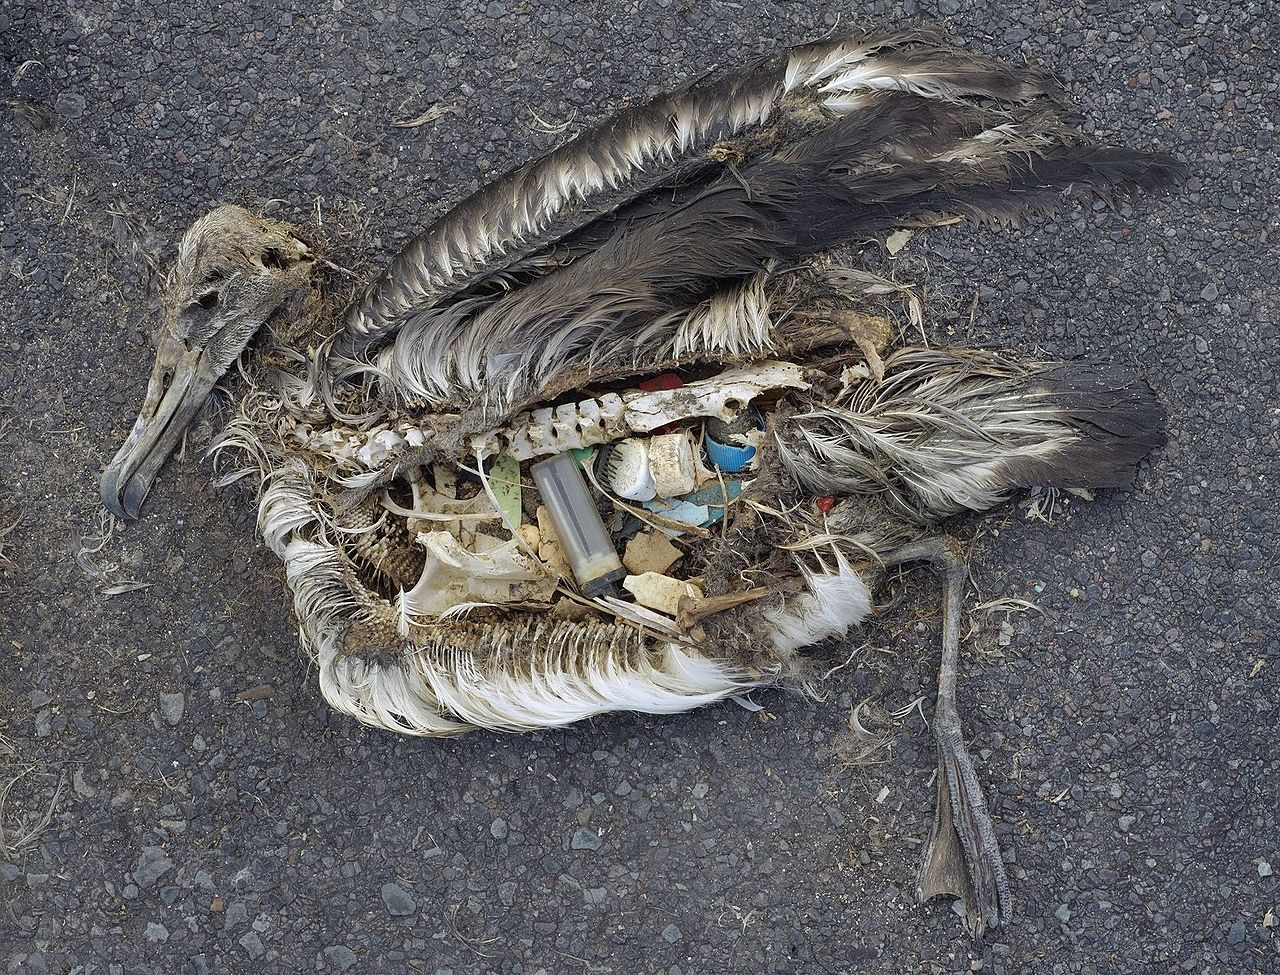
\includegraphics[height=6cm]{graphics/ChrisJordan-Albatross.jpg}
  \caption{Chris Jordan, Albatross at Midway Atoll Refuge, 2009}
  \label{fig:ChrisJordan_Albatross}
\end{figure}

The unaltered stomach contents of a dead albatross chick photographed on Midway Atoll National Wildlife Refuge in the Pacific in September 2009 include plastic marine debris fed the chick by its parents.

Using spare narration and stunning imagery, Chris Jordan's feature film MIDWAY explores the plight of Laysan albatross plagued by the ingestion of our plastic trash. Both elegy and warning, the film explores the interconnectedness of species, with the albatross on Midway as a mirror of our humanity.

Even if garbage leave outs our life, we do not care about the results of it. And it is captured by the works of Chris Jordan.In this photo series it captures 


% Effect of plastic on wildlife in Antartica.
% Her ne kadar biz çöpü attıktan bizim hayatımızdan çıksa da yok olmuyor. Sadece başka bir yerlere gidiyor. Mesela kuşların midelerine. Chris Jordan'ının imageları bunu çok da güzel açığa çıkartıyor. Bizim çöpleriminde habersiz hayvanlar bunları yiyorlar. Bir yandan ürettiğimiz ürünler ile kaynakları tüketirken bir diğer yandan ise artıklarımız diğer yaşanları tüketiyor. Dikkat çekmek istediğim nokta aslında ekolojik hassasiyetlerden çok aslında elimizde avucumuzda ne varsa onları tüketiyor olmamız. Karşı durduğum nokta ise tam olarak burası. 


%****************************************

% First one is actually is to analyze what is trash? Because I am using trash material and what is point of view of scholars to the trash. Realizing the potentials of it. Also the difference comes from the working on virgin object and trash object. Çöp kendi geçmişini falan taşıyor. Yeni blank bir şey değil aslında. Boş bir kağıda resim yapmak ile başka bir kağıdın üzerine resim yapmak arasındaki fark gibi bu. If trash has multiple life than these research will somehow reveal it. It is actually research on trash. I guess it is missing? Yani sanatın dilini genişleten yeni bir soru gündeme atan bir iş değil. I need to set a purpose for the theory chapter. Or it is a just a background chapter?

% Genel anlayışın tersine --- çöpün değersiz, iğrenç, uzak durulması algısına --- karşıt değerli olabileceğini, bir kaynak olduğunu iddia ediyorum, tıpkı bu sanatçıların işleri gibi. Genel göürüşe meydan okuyorum. Sizleri gerçekten bunların değerli bir şeyler olduğuna vs. ikna etmeye çalışacağım

% Ben bu bu bu methodlarla bu işi geliştirdim. Bir dert var o dert üzerine (şu yöntemlerle) sorgulamalar yapıyorum. 

%........................................





%****************************************
% Rubbish: the archaeology of garbage. rathje1992rubbish
% [Refreshed ideas] Garbage project's findings have supplied a fresh perspective on what we know --- and what we think we know --- about certain aspects of our lives. p.24

% The basic methods of garbage disposal are four: dumping it, burning it, turning it into something that can be useful (recycling), and minimizing the volume of material goods. p.33

% ancient peoples p.33

% fast food packaging. p.97

% human behavior p.55 can you tell a lot about the customers from their garbage?

%p.191-192 people tend to think of "recycling" as a relatively modern conceit that has only recently gained broad public acceptance, and whose practical benefits have only just began to be realized. Recycling itself is probably as old as --- indeed, seems to be a fundamental characteristic of --- human species.

%p.209 The reuse of paper, for example, involves processes that generated a considerable amount of hazardous waste. In order to recycle newspapers, magazines, and, indeed, any printed paper, the paper must first be de-inked. At the end of the de-inking process one is left with essentially two products: on the one hand, de-inked fiber that will be turned into new paper; and on th other, a large quantity of toxic sludge.
%........................................


%****************************************
% trasformations 

% during great depression, I learned firsthand about frugality as a child during ww2. my family carefully folded the wrapping paper from gifts to reuse on other occasions. p.8

% p11. for decades we've taken for granted used cars and old houses. Is there anyone alive who has always lived in new houses or driven only new cars?

% p.11 Economics has always been a factor in recycling. 

% p.12 recycling is not limited to folk art. 

% Use of recycled materials is not new, not is it exclusive to the united states. p.18

% p.22 Material, meaning, and memory --- these are artists' reasons for using found objects.

% p.48 recycling may be the most wasteful activity in modern America --- a waste of time and money, a waste of human and anutral resources. john tierney, "What a Waste," seattle postintelligencer...
%........................................





\paraphrase{The names we give this material ---waste, garbage, refuse, trash, rubbish--- have pejorative definitions. Worthless. Rejected and useless matter of any kind. Unimportant. \cite{zimring2012encyclopedia}}



[Trashing Habits] Various objects become trash after their primary functions consumed. People do not care the package of the objects that they buy. They buy the coffee not the cup of it. After coffee finished the life of cup also finishes. They are actually packages that are used to carry or protect other materials. After real material used these packages became valueless (or useless).



[LIFE OF OBJECTS] Objects life time in the nature is more than human being. People use them for just 5 minutes. However, they continue to exist on the nature through the years becauseof they are the result of highly complex industrial production methods and They are not easily decomposable items in the nature. 


% Şu anda lazım değil.
[Biodegradable] \comment{Biodegradable matter is material capable of being decomposed by bacteria or other biological means. Biodegradable  matter usually consists of organic materials such as plant, animal, and other substance matter originating from living  organisms. It has the ability to be broken down into smaller, harmless products by way of the action of living organisms.  The term is often used in relation to ecology, garbology, and waste management. Biodegradable products are often associated with perishables (products, food, and waste materials subject to death or decay). The term biodegradability of a product  refers to its disposition to disintegrate as the result of natural processes.}



% Bu kısma hiç gerek yok.
[Different types of trash] The complexity of produced trashes of societies is increasing. For example developed countries that have nuclear plant generates radioactive wastes which highly hazardous for the environment is never exist previous societies. Think batteries and so on.  It can be thought that when the complexity of trashed increased required effort to repair, reuse and recycle is also increase. Therefore for the ones that have no complex tools it is becoming harder to reuse objects. In other words objects become more complex their re-usage becomes less likely.  Different production process generates different types of trash. According to production process, decomposition process\ldots The approach to the different type of trash will be different. In other word if trash is a result of classification of objects, it can be easily extracted that there is classification inside of it. There are some trashes that are more close to the people. More easy to convert them. more easy to regain to the society. 



%****************************************
% UPCYCLING:
% Burada da upcycling kullanıyor aslında. http://www.gwynethleech.com/cups/suspended
% Raw+Matrial=Art burda da upcycling deniliyor.
%
% RECYCLING:
% recycled, re-seen book.
%........................................




\todo{throwaway spirit (vance packard)}

[Unprofitable, Value, Definition] Waste is considered as something useless, something no longer has value; something sufficiently degraded so that the cost of reclaimation seems higher than the cost of disposal, in other words, something unprofitable. 

[Determination] \paraphrase{The value of things rises and diminishes according to the work they do or the feature imagined for them, in other words, to their potential realized in time. Waste by Willian Viley.}

We are very good at producing waste as well as hiding our garbage. 

[Question] Is it trash or trashed? Is it waste or wasted?

% CHANGE
\paraphrase{In the late twentieth century, in the context of increasing environmental awareness, this consciousness has altered yet again, and waste has ‘been revalued and recoded from rubbish to recyclable resource, it has moved from the bin to the compost heap, it has insinuated itself into our lives in different ways and with different effects’ (Hawkins 2006: 5).}

% Reference from Identity, mobility and the throwaway society
% Resource is here: mmmacleo2005.pdf (throw away culture ile ilgili.) (Çünkü ben bunun ürününü kullanıyorum.)
\paraphrase{In this thesis the undeniable matter of waste, itself pressing, urgent and excessive, is used to infer the presence of a society defined by its generation; a society ceaselessly discarding and abandoning its surplus as excess, as part of an endless desire for the new. Morally corrupt and unequivocally environmentally damaging, the rhetoric of the throwaway society classifies discarding as intrinsically bad and commands us to assume control of our wasting, suggesting the adoption of heightened regulatory practices around disposal as the means to ensure that we clean-up our act. The thesis, however, lacks depth and provenance. It is, actually, glib. Indeed, to infer the presence of a throwaway society from contemporary levels of waste generation is problematic for at least four reasons.}



%****************************************
% MOVE TO CHAPTER 4
% HAKAN GÜRSU, ZIZEK
% Buraya aslında bir de Hakan Gürsu koymak gerekli olabilir. Yani aslında kendisi pek de sanatla ilgili bir laf etmiyor. Ama aslında tükettiğimiz onlarca şeye karşı bir tavır yaklaşım sergiliyor. Bu yüzden theory kısmında yer alabilir. Bu çöpün içinde boğulacağımızdan bahsediyor. Onu dönüştürmek gerekliliğinden yeteneğinden bahsediyor.
%........................................


%****************************************
% TEZ STATEMENT. Dönüştürme
% Ya gerçekten çöpü dönüştürüyorlar ya da çöpe dair düşünceleri dönüştürüyorlar, ve bunu ele alırken aslında heykel, kolaj, fotoğraf gibi şeylerden yararlanıyorlar ama aslında ortaya koydukları şey bir sanatsal eylem. veya bunu sanatsal eylem bağlamında ele alabiliriz.


% Dönüştürme çok temel bir şey ve çöpe çok bağlı. Çünkü değeri sıfıra inmiş bir şeyden bahsediyoruz.
%........................................


as trash live longer than human being, next generations have to cope with previous generations trash. 




[Inspired Works] There are some works that inspire me a lot when developing the work. They are not actually trash related works therefore I put them in different section and here before the details of my work. However the previous chapter has also very inspirational contributions to the my work. They helped the understand the topic and develop an approach to the topic. In this section some projects are mentioned and their methodologies are explained. How are these works effected my work. What is the relationship between them? (Maybe all of them can be explained only the related part of it.)




Recycle the Classics, BY DORIS SOMMER

Trash as History/Memory, Encylopedia, bullock2012trash

John Scanlan's book, On Garbage shows how western progress always has cleared away and discarded what went before; not only material waste but also knowledge. He believes that by examining our garbage we can gain useful insight into the condition of contemporary life.

Book: Recycled, Re-Seen: Folk Art from the Global Scrap Heap






%****************************************
% RESOURCES:
%
% Plagiarism check: http://mashable.com/2012/08/29/plagiarism-online-services/
% What is Plagiarism: http://www.plagiarism.org/plagiarism-101/what-is-plagiarism
%
% How to cite epigraph: http://blog.apastyle.org/apastyle/2013/10/how-to-format-an-epigraph.html
%
% Artist ve artist statementlar için kaynak:
% - http://www.amandadonahue.com/artist-statement/
% - http://www.smfa.edu/cyclo-show
% - http://www.gwynethleech.com/statement
%........................................





%**************************************
% HERE Same sample phrases are listed you can use them:


% The work that follows is divided into three sections


% The artist thinks, acts, performs music, and writes outside the framework that society has created.


% This thesis takes a rather different approach to the resonant possibilities of discarded things. It looks to philosophical ideas and our entangled experiences of things, time and stories, which need to be traversed in order for a discarded object to be called ‘waste’.


% I also want to suggest a different way of considering trash. Maybe art maybe suggest an alternative way of seeing.


% I’d like to criticize a set of concepts or ways of thinking about discarded things that to me just don’t seem quite adequate.


% In an effort to expand art activism's capacity to create real social change, this article will (1) examine the theoretical framework behind art activism and art's efficacy in accessing emotional pathways; (2) explicate ways to strategically approach art activism through the use of specific case studies; and (3) explain one practical form of art activism-theater-based conflict resolution-that is transforming the ways communities are addressing social injustice.


% This thesis is written as a study of the socio-economic change that is currently happening in Serbia, but it’s a study that critically engages with everyday materials that provide the basis for change, rather than the economic development philosophies that are practiced through policy. 


% What specific social issues are you trying to address through Labyrinth?

% The discussions (mentioned discussion are also formed the thesis project entitled ... )


% Aim of this thesis is ...


% There has been a recent spate of artistic work focusing on (over-)consumption using the lens of disposal and discard.


% as a reaction to the consumerist society.


% \ldots is the concern of this study which aims to \ldots


% The aim is not to practice Antiquarian Avant-Garde techniques as a puritan form of photography, but rather to envision new means of photography.


% The aim of the thesis paper is to historically, socially and theoretically contextualize a student's work. The written thesis documents and informs the development and resolution of each student's artistic practice during the MFA program.


% The main aim of the current study was to produce an initial conceptual model that explains 


% The topic of recycling, presented in this issue, is the "re-use" of materials, objects and structures, for different purposes, and in different ways from their original uses, in order to build or re-build, to provide possible solutions to problems related to the environment, and to manage waste more intelligently. Tyres, containers, bottles, cans, CD-ROMs and even keyboards, can find new and unexpected uses in experimental architecture, exhibition pavilions, or low-cost housing. With recycled objects, one can build anti-seismic and energy efficient houses. Recycled materials can contribute towards building shelters to meet the needs of people affected by disasters. There are many topics connected to recycling, and they vary depending on the objects that one wishes to recycle and how they will be put to use. Used tyres find many applications in REfunc architecture and the Bohlin-Cywinski-Jackson studio. Dorte Mandrup transformed a piezometer into the supporting structure for apartments built with standardized modules. David Hertz reused the wings of a 747 as roof for a villa in Malibu. TYIN Tegnestue architects restored a building with recycled materials, mainly found on location. Yatin Pandya and Footprints E.A.R.T.H. built an activity centre in Ahmedabad using items that were considered as rubbish to their original owners. James & Mau and Infiniski designed fashion homes with recycled containers. The same kind of containers were used by MacArthur Studio and Means & Wells, to build a travelling exhibition pavilion. The GAD. In London, Folke Koebberling and Martin Kaltwasser constructed an experimental theatre using only recycled materials. The panorama that emerges shows the extreme heterogeneity of the work, materials and techniques, the intuitive approach and the infinite possibilities offered by recycling. All of these projects highlight the importance of the construction process as an opportunity for learning and discussion. 

% In light of this argument

% To frame a discussion, narrow down the topic

%........................................


My work relation with the other works.

(My work needs to be considered in the context of art. I need to focus on the notebooks establish with art.)

sanki çöplerden bir şeyler yapmak bir şeyleri ispatlamak gibi gözüküyor. Ya da gene bir yetenek gibi gözüküyor. Bulunmaz kumaş misali. Yok abi kimsenin başaramadığı şeyi başarıyorum gibi bir şey yok. Ben ilgilinilmeyenle ilgileniyorum.

